\documentclass{article}

% Packages
\usepackage{geometry}
\usepackage{graphicx}
\usepackage{lipsum}
\usepackage{tcolorbox}
\usepackage[portuguese]{babel}
\usepackage[margin=4cm]{caption}

\tcbset{%any default parameters
    toprule=3mm,
    arc=2mm,
    bottomtitle=2mm
}

% Page setup
\geometry{a4paper, margin=2cm}

\begin{document}

\thispagestyle{empty} % Remove page number from first page

\begin{figure}[t]
    
\includegraphics[width=3cm]{imagens/logo-puc-minas.png}
    \hspace{0.02\textwidth}
    \vline%
    \hspace{0.04\textwidth}
    
\includegraphics[width=3cm]{imagens/logo-icei.jpeg}
\end{figure}

\hrulefill%
\vspace{\baselineskip}

\Large\noindent
\textbf{Pontifícia Universidade Católica de Minas Gerais} \\
\textbf{Instituto de Ciências Exatas e Informática} \\
\textbf{Departamento de Engenharia de Computação}

\begin{center}
    \vfill
    \Huge\textbf{Relatório do Laboratório 5} \\
    \vspace{0.5cm}
    \Large\textbf{Fonte Regulada com Diodo Zener} \\
    \vspace{1cm}
    \large \textbf{Professor}: Bruno Luiz Dias Alves de Castro \\
    \vspace{0.5cm}
    \large Bruno Luiz Dias Alves de Castro \\
    \large Bruno Luiz Dias Alves de Castro \\
    \large Bruno Luiz Dias Alves de Castro \\
    \vfill
    \large Belo Horizonte \\ Campus Coração Eucarístico \\
    \vspace{\baselineskip}
    \large \today
\end{center}
\newpage

\thispagestyle{empty}
\tableofcontents
\newpage

\section{Introdução}

Durante o Laboratório 5, fomos encargados em trabalhar com o diodo zener. O diodo zener (também conhecido com diodo regulador de tensão), tem funcionamento semelhante à um diodo convencional, porém é projetado para conduzir em regime de condução inversa. \\

Mais sobre o diodo zener é apresentado na Secção \ref{zener}

\subsection{Objetivos}
Ao final do experiemento, devemos ser capazes de:


\begin{tcolorbox}
    \begin{enumerate}
        \large
        \item Realizar medições de corrente e tensão utilizando um multímetro;
        \item Analisar o efeito do diodo zener como regulador de tensão em fontes de alimentação e suas limitações;
        \item Analisar formas de onda utilizando o osciloscópio.
    \end{enumerate}
\end{tcolorbox}

\section{Experimento}

\subsection{Materiais e equipamentos necessários}

\begin{tcolorbox}
    \begin{itemize}
        \large
        \item 1 Osciloscópio;
        \item 2 Multímetros;
        \item 1 Módulo de fonte de CC;
        \item Conjunto de cabos de teste.
    \end{itemize}
\end{tcolorbox}

\subsection{Teoria}
\subsubsection{Diodo Zener}
\label{zener}

Os diodos Zener são projetados para operar de forma estável sob condições de ruptura reversa, ao contrário dos diodos comuns. Na curva característica de um diodo Zener, a área do lado esquerdo do gráfico (área de polarização reversa) é onde a tensão permanece quase constante, independentemente das mudanças na corrente após atingir a tensão Zener. Esta tensão de ruptura reversa é a tensão Zener. Essencialmente, a tensão permanece estável mesmo quando a corrente reversa aumenta, permitindo que o diodo atue como um regulador de tensão, protegendo o circuito contra sobretensão. Quando a corrente flui nesta região de ruptura, o diodo Zener mantém uma tensão de saída estável, o que é ideal para aplicações de regulação de tensão.

\begin{figure}[h!]
    \centering
    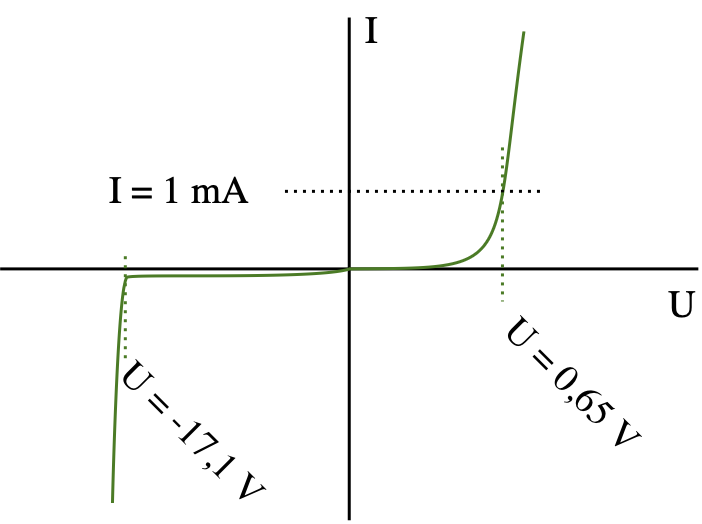
\includegraphics[width=8cm]{images/diodo-zener.png}
    \caption{
        Gráfico corrente x tensão de um diodo zener \\ \\
        \tiny
        Por Filip Dominec - Obra do próprio, CC BY-SA 3.0, https://commons.wikimedia.org/w/index.php?curid=1440010
    }
\end{figure}

\section{Parte Prática}

\subsection{Questão 3}

\begin{tcolorbox}[title=\large Questão 3, colback=red!5!white, colframe=red!75!black]
    \large
    alimentar o circuito e medir os valores da corrente e tensão média na carga
\end{tcolorbox}

Os seguintes valores foram medidos durante o experiemento:

\begin{center}
    \begin{tcolorbox}[width=0.6\textwidth]
        \centering
        $I_{DC} = 135mA$
        \hspace{2cm}
        $V_{DC} = 28,86V$
    \end{tcolorbox}
\end{center}

\subsection{Questão 4}

\begin{tcolorbox}[title=\large Questão 4, colback=red!5!white, colframe=red!75!black]
    \large
    utilizando os valores medidos no item anterior calcular o valor da resistência de carga e comparar com o valor indicado no módulo Fonte CC. Explicar possíveis diferenças;
\end{tcolorbox}

Valor de resistência encontrado:
    
\begin{center}
    \begin{tcolorbox}[width=0.3\textwidth]
        \centering
        $R_{C} = 213,77\Omega$
    \end{tcolorbox}
\end{center}

\textbf{Resposta}: Essa diferença pode ser devida às tolerâncias dos componentes ou à precisão do equipamento de medição. A resistência de um componente pode variar dentro de uma determinada percentagem do seu valor nominal, que é representado pela série de tolerâncias do componente. Além disso, as condições ambientais, como a temperatura, podem afetar a resistência medida.

\subsection{Questão 8}

\begin{tcolorbox}[title=\large Questão 8, colback=red!5!white, colframe=red!75!black]
    \large
    desenhar as formas de onda das tensões no capacitor C3 e na carga no eixo ao lado. Comentar as formas de onda obtidas;
\end{tcolorbox}

\begin{figure}[h!]
    \centering
    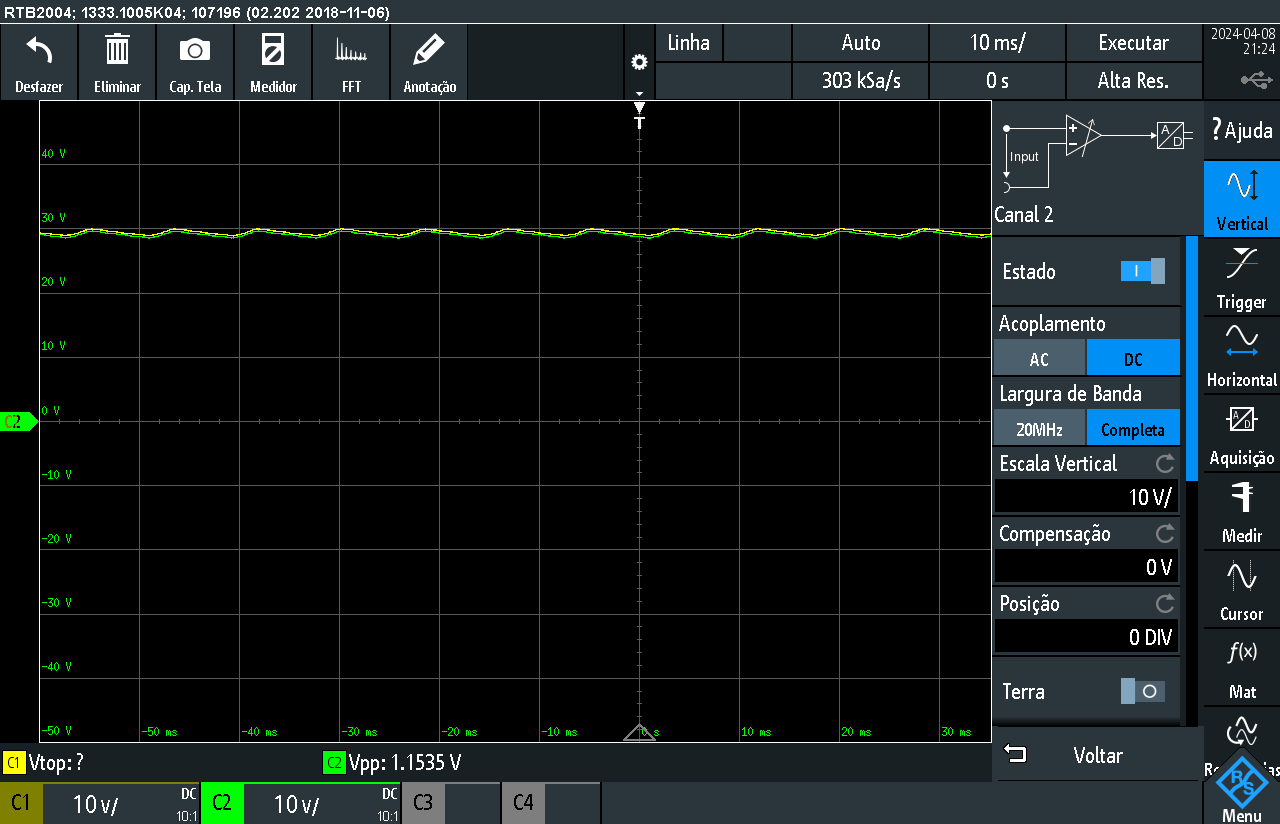
\includegraphics[width=12cm]{images/SCR06.PNG}
    \caption{Osciloscópio, primeira montagem}
\end{figure}

\subsection{Questão 12}

\begin{tcolorbox}[title=\large Questão 12, colback=red!5!white, colframe=red!75!black]
    \large
    analisar em função do fator de ripple na carga qual o efeito da inclusão do diodo zener no circuito retificador;
\end{tcolorbox}

\textbf{Resposta}: A inclusão do diodo Zener no circuito retificador serve para estabilizar a tensão de saída, reduzindo o ripple. O diodo Zener mantém a tensão sobre a carga constante ao seu valor de Zener, mesmo com flutuações na tensão de entrada ou carga.

\subsection{Questão 13}

\begin{tcolorbox}[title=\large Questão 13, colback=red!5!white, colframe=red!75!black]
    \large
    ligar agora o canal 1 do osciloscópio para observar a forma de onda da corrente no diodo zener. Para isso ligar os terminais do osciloscópio no resistor R3 de 1$\Omega$. Como o valor do resistor é conhecido, basta dividir o valor do fator de escala do osciloscópio (Volts/divisão) por $1\Omega$ para que se tenha um fator de escala graduado em Ampère/divisão. Fazer isso e anotar o fator de escala encontrado;
\end{tcolorbox}

\begin{center}
    \begin{tcolorbox}[width=0.4\textwidth, title=\large Fator de escala em Ampere/div]
        \centering
        $50mA$
    \end{tcolorbox}
\end{center}

\subsection{Questão 14}

\begin{tcolorbox}[title=\large Questão 14, colback=red!5!white, colframe=red!75!black]
    \large
    observar a forma de onda na carga e em R3 simultaneamente no osciloscópio. Tire conclusões sobre a condução do diodo. Desenhar as formas de onda da corrente IZ e da tensão na carga no eixo ao lado. Anotar os dois fatores de escala;
\end{tcolorbox}

\begin{figure}[h!]
    \centering
    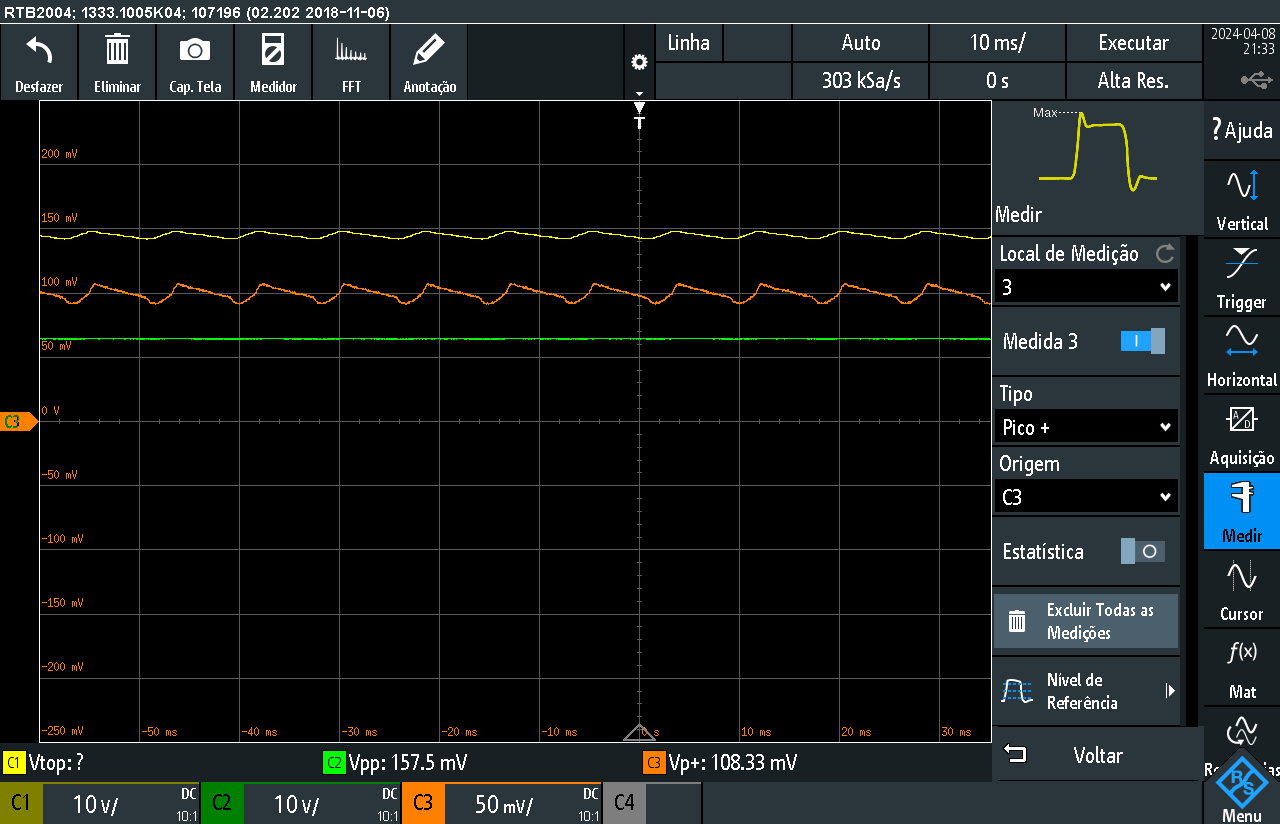
\includegraphics[width=12cm]{images/SCR07.PNG}
    \caption{Osciloscópio, segunda montagem (capacitor C3)}
\end{figure}

\subsection{Questão 17}

\begin{tcolorbox}[title=\large Questão 17, colback=red!5!white, colframe=red!75!black]
    \large
    religar o módulo Fonte CC e medir a corrente e tensão na carga;
\end{tcolorbox}

Os seguintes valores foram medidos durante o experiemento:

\begin{center}
    \begin{tcolorbox}[width=0.6\textwidth]
        \centering
        $I_{RL} = 60mA$
        \hspace{2cm}
        $V_{RL} = 12,88V$
    \end{tcolorbox}
\end{center}

\subsection{Questão 19}

\begin{tcolorbox}[title=\large Questão 19, colback=red!5!white, colframe=red!75!black]
    \large
    desenhar as formas de onda da corrente $I_Z$ e da tensão na carga no eixo ao lado. Anotar os dois fatores de escala. Tire conclusões sobre a condução do diodo.
\end{tcolorbox}

\begin{center}
    \begin{tcolorbox}[width=0.4\textwidth, title=\large Fatores de escala (Ampere/div)]
        \centering
        $I_{In} = 50mA$
        \hspace{2cm}
        $I_{Z} = 100mA$
    \end{tcolorbox}
\end{center}

\begin{figure}[h!]
    \centering
    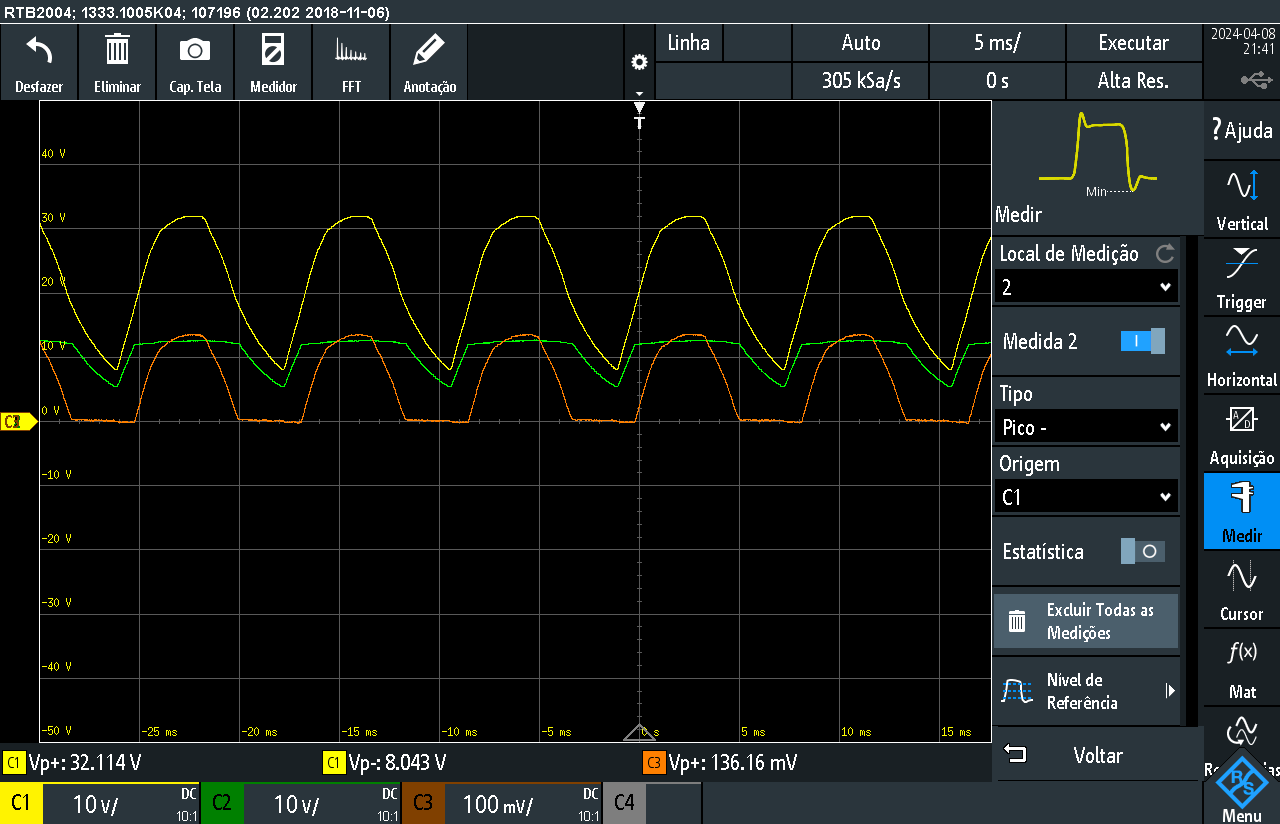
\includegraphics[width=12cm]{images/SCR08.PNG}
    \caption{Osciloscópio, segunda montagem (capacitor C1)}
\end{figure}

\subsection{Questão 20}

\begin{tcolorbox}[title=\large Questão 20, colback=red!5!white, colframe=red!75!black]
    \large
    medir a corrente e tensão na carga;
\end{tcolorbox}

Os seguintes valores foram medidos durante o experiemento:

\begin{center}
    \begin{tcolorbox}[width=0.6\textwidth]
        \centering
        $I_{RL} = 50,5mA$
        \hspace{2cm}
        $V_{RL} = 10,84V$
    \end{tcolorbox}
\end{center}

\section{Questionário}

\subsection{Questão 1}

\begin{tcolorbox}[title=\large Questão 1, colback=red!5!white, colframe=red!75!black]
    \large
    qual a limitação de uso do diodo zener como regulador no circuito estudado?
\end{tcolorbox}

O diodo Zener tem uma limitação de dissipação de potência; ele só pode dissipar uma quantidade finita de energia na forma de calor antes de ser danificado. Se a corrente que passa por ele for muito alta, ele pode superaquecer e falhar. Portanto, o diodo Zener no circuito é limitado pela sua capacidade máxima de corrente e pela potência que pode dissipar de forma segura.

\subsection{Questão 2}

\begin{tcolorbox}[title=\large Questão 2, colback=red!5!white, colframe=red!75!black]
    \large
    pesquisar na Internet alguns fabricantes e modelos de diodos zener com tensão de 5,1V, 8,2V, 9V e 12V
\end{tcolorbox}

\textbf{UNIT Electronics}:
\begin{itemize}
\large
    \item 1N4733A: Diodo Zener de 5,1V
    \item 1N4738A: Diodo Zener de 8,2V.
    \item 1N4742A: Diodo Zener de 12V
\end{itemize}

\vspace{\baselineskip}

\textbf{Micro Commercial Co (DigiKey)}:
\begin{itemize}
\large
    \item 3SMAJ5918B-TP: para 5.1V 
    \item 3SMAJ5923B-TP: para 8.2V
\end{itemize}

\vspace{\baselineskip}


\textbf{Vishay Semiconductors}:
\begin{itemize}
\large
    \item PLZ9V1A-G3/H: para 9v
\end{itemize}

\subsection{Questão 3}

\begin{tcolorbox}[title=\large Questão 3, colback=red!5!white, colframe=red!75!black]
    \large
    desenhar a curva característica do diodo zener mostrando todas as correntes e tensões de interesse.
\end{tcolorbox}

\subsection{Questão 4}

\begin{tcolorbox}[title=\large Questão 4, colback=red!5!white, colframe=red!75!black]
    \large
    explicar a função da ponte retificadora, do capacitor e do resistor $R_2$ no circuito mostrado na Figura 10.
\end{tcolorbox}

A ponte retificadora transforma a corrente alternada em contínua pulsante. O capacitor suaviza a tensão pulsante, reduzindo o ripple. O resistor $R_2$ limita a corrente para o diodo Zener, protegendo-o de sobrecorrente

\end{document}